\chapter{Oprogramowanie}
W obecnych czasach praca w eksperymencie fizyki wysokich energii nieodzownie łączy się z programowaniem. Każdy element pracy zaczynając od zbierania danych poprzez selekcja przypadków po analizę wykonywany jest poprzez napisane przez członków kolaboracji oprogramowanie. Dlatego tak ważnym elementem w pracy są umiejętności programistyczne. Poniższy rozdział ma na celu przedstawienie narzędzi używanych podczas analizy, która to jest opisywana przez niniejszą pracę magisterską. Ponadto pokrótce przedstawione będą techniki tworzenia oprogramowania, na których autor starał się oprzeć swoje badania.

Rozdział ten zaczyna się od przedstawienia dwóch języków programowania, w których napisano oprogramowanie będące integralną częścią pracy magisterskiej. Następnie przedstawione będą narzędzia programistyczne używane przez przez kolaboracje LHCb, wykorzystane w analizie. 

\section{Root}
Root \cite{ROOT} jest zorientowaną obiektową platformą programistyczną (ang. framework) napisaną w języku C++ na potrzeby Fizyki Wysokich Energii rozwijana przy ośrodku CERN, oraz rozpowszechniana na licencji LGPL. Głównymi zaletami środowiska są bardzo rozwinięte biblioteki ułatwiające statystyczną analizę danych. ROOT umożliwia między innymi:
\begin{itemize}
 \item tworzenie oraz analizę histogramów, zarówno jedno jak i wielowymiarowych,
 \item dopasowywania krzywych do danych przy użyciu różnych metod, między innymi metody największej wiarygodności, czy minimalizacji funkcji $\chi^2 $,
\item bardzo wydajne,pod względem ilości zajmowanego miejsca, przechowywanie danych, w tym celu utworzone i zoptymalizowane obiekty o nazwie Ntuple,
\item korzystanie z zaawansowanych operacji matematycznych np. rachunek na macierzach, czterowektorach,
\item równoległe przetwarzanie danych
\item prace z specjalnie stworzonym interpreterem 
\item wizualizację 3D
\item tworzenie plików w wielu najpopularniejszych formatach graficznych typu  PostScript, PNG, SVG, JPG czy GIF
 \end{itemize}
 \subsection{RooFit}
 Napisać o rooficie z manuala
 \section{Gaudi}
 Eksperyment Fizyki Wysokich Energii produkuje rocznie peta bajty danych, które muszą zostać zrekonstruowane, a następnie zanalizowane w celu produkcji końcowych fizycznych rezultatów. Czas życia takiego eksperymentu wynosi wiele lat w związku z tym oprogramowanie rozwijane przy nim musi mieć możliwość dopasowania do zmian technologii. Drugim ważnym wymaganiem dotyczącym oprogramowania jest elastyczność, możliwość wykorzystania w wielu dziedzinach, począwszy wydobycia interesujących przypadków z tła- algorytm HLT, poprzez rekonstrukcję po analizę fizyczną. Jednym z powodów owych wymagań jest ujednolicenia całego oprogramowania używanego przez ludzi pracujących przy eksperymencie, co ułatwia  zajmowanie się wieloma aspektami pracy, wystarczy jednorazowe nauczeniu się zasad tworzenia oprogramowania.  \\
Wychodząc na przeciw tym wymaganiom stworzono architekturę GAUDI\cite{GAUDI}. Podczas tworzenia architektury została podjęta decyzja o rozdzieleniu ``danych'' od ``algorytmów''. Poprzez dane rozumiano przykładowo składowe pędów oraz energie cząstek natomiast algorytmem może być funkcja wyliczająca masę inwariantną oraz dopasowująca odpowiednią krzywą. Algorytmy mogą tworzyć nowe typy danych. Natomiast dane dzielimy na trzy typy:
\begin{itemize}
 \item Event data- dane otrzymane z zderzenia protonów oraz ich pochodne,
 \item Detector data opisujące aparaturę detekcyjną, używane do interpretowania danych pomiarowych ( struktura, geometria, parametry środowiskowe),
 \item Dane statystyczne- wynik przetwarzania ww danych (histogramy, Ntuple).
\end{itemize}
 \begin{figure}[h]
 \centering
 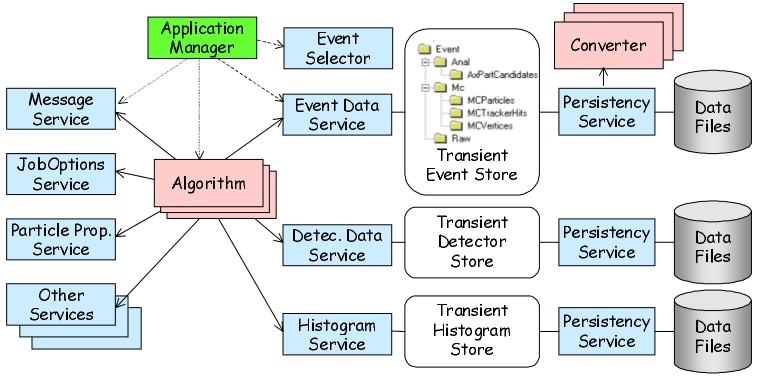
\includegraphics[scale=0.8]{rozdzial4/GAUDI.jpeg}
 % GAUDI.jpeg: 767x379 pixel, 96dpi, 20.29x10.03 cm, bb=0 0 575 284
 \caption{Schemat blokowy architektury GAUDI\cite{GAUDI}}
 \label{rys:GAUDI architektura}
\end{figure}

Rysunek \ref{rys:GAUDI architektura} przedstawia główne elementy architektury oraz ich interakcję, przy czym nie wchodzi w szczegóły dotyczące zastosowanych klas. \\
Dzięki swojej elastyczności GAUDI jest podstawą oprogramowania używanego w LHCb oraz ATLAS.
Mimo iż kod GAUDI'ego napisany jest w języku C++ to konfiguracja wykonywane jest przy użyciu skrpytów Python'owskich.

\section{Da Vinci}

